% !TeX spellcheck = en_GB
\documentclass[a4paper]{article}
\usepackage[english]{babel}
\usepackage[utf8x]{inputenc}
\usepackage{amsmath}
\usepackage{booktabs}
\usepackage{graphicx}
\usepackage{hyperref}
\usepackage{nicefrac}
\usepackage{float}
\usepackage{subfigure}
\usepackage{enumitem}
\usepackage{titling}
\usepackage{algorithm2e}
\usepackage{lipsum}

 
% Font and spacing

\usepackage{lettrine}
\usepackage{color}


\title{ \huge Neural Networks: \\
	Project Report.}
\author{Irvin Aloise, Mirco Colosi\\
	\textit{Sapienza University of Rome}}

\begin{document}
	
	\maketitle
	
	\section{Introduction}
	\lettrine[nindent=0em,lines=2]{M}{idi} databases are still very popular nowadays and the scientific community is always improving the way in which it is possible to categorize them. MIDI - which stands for \textit{Musical Instrument Digital Interface} - is a technical standard that allows to connect and make them communicate properly several musical tools, e.g. instruments, digital equipment and computers [ref. https://en.wikipedia.org/wiki/MIDI]. It is composed by messages containing informations about \textit{notation}, \textit{pitch}, \textit{velocity}, \textit{control signals} - that describe parameters like vibrato or the volume - and \textit{clock} signals in order to synchronize the tempo of all the instruments.
	
	With the diffusion of machine learning approaches, those classification methods are always more powerful and precise, taking advantage of MIDI informations together with other audio features, in order to achieve categorization of the tracks by \textit{author}, \textit{genre}, \textit{style} and so on. 
	
	In this paper, instead, it has been used a more general approach: it has been designed and developed a mechanism that measures the similarity between tracks and, given a new instance returns the author which mostly suits that instance - chosen between the authors available in the training set. To do that, we used a \textit{universal} similarity metric based on \textbf{Kolmogorov complexity} [ref: LI, Ming, et al. The similarity metric. IEEE transactions on Information Theory, 2004, 50.12: 3250-3264.]. The peculiarity of this approach is that can be employed potentially on every kind of file with no modification and without the need of time expensive calculations for extracting audio features. Then, once that a similarity measure is retrieved, a simple \textit{k-NN} has been employed to classify new instances.
	
	The remaining of the document is organized as follows: in Section 2 a brief overview of the related approaches is given; Section 3 describes the methodology used in this project together with some results; finally in Section 4 are reported conclusions and possible future improvements.
	
	
	\section{Related works}
	\lettrine[nindent=0em,lines=2]{M}{}ost of the works in the literature try to classify MIDI songs by \textit{genre}. This because generally datasets are stored by author but recognize the style could be useful in automated platforms, for example to suggest a new song related to the one that we are listening. 
	
	For example, \textbf{Basili et al} [ref: Basili, Roberto, Alfredo Serafini, and Armando Stellato. "Classification of musical genre: a machine learning approach." ISMIR. 2004.] use some \textit{coarse-grain features} in order to classify MIDI files by genre. Those features are basically provided directly by the MIDI file, in order to evaluate how good MIDI describe symbolic music; they are the following ones:
	\begin{itemize}
		\item Melodic intervals
		\item Instruments
		\item Instrument classes and drumkits
		\item Meter and time changes
		\item Note extension
	\end{itemize}
	Those features are given as input to several machine-learning algorithm - \textit{Naive Bayes}, \textit{VFI}, \textit{J48}, \textit{PART}, \textit{NNge} and \textit{JRip} - to extract a genre prediction for new MIDI instances.
	
	\begin{figure}[!h]
		\centering
		\label{fig:audio_and_NCD}
		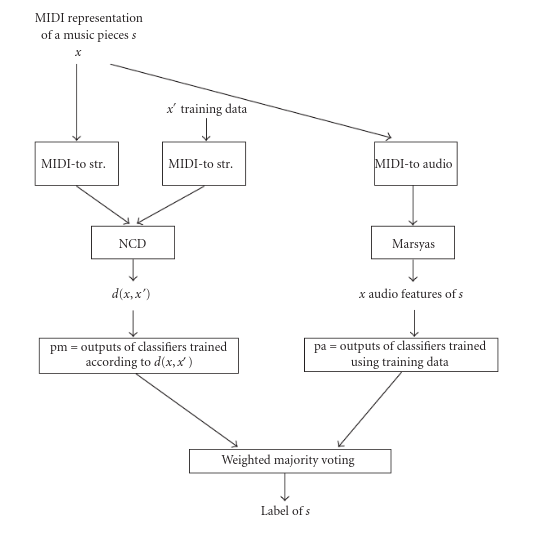
\includegraphics[scale=0.5]{misc/audio_and_ncd.png}
		\caption{A block scheme representing Cataltepe et al.'s approach}
	\end{figure}
	
	\textbf{Chet} in his work [ref: Gnegy, Chet N. "Classification of Musical Playing Styles using MIDI Information."] instead tries to return a \textit{style} classification of the instances, intended as a functional description of a specific instruments in a song. More precisely, the styles used are the following: 
	\begin{itemize}
		\item \textbf{Bass}: the song has a predominant single line of deep tones and the other harmonic structure are just supporters.
		\item \textbf{Lead}: a melodic line, e.g. vocal performance or guitar solo.
		\item \textbf{Rhythm}: in general represented by repeated chords that give the rhythmic structure to the melody.
		\item \textbf{Acoustic}: this style is characterized by multiple individual notes - or melody lines - often performed on the same instruments.
	\end{itemize}
	A large variety of audio features is used in this work, spanning from simple statistics - \textit{mean pitch}, \textit{pitch standard derivation} and many others - to very complex ones - \textit{coverage}, \textit{liricality} and several others. Many different machine-learning algorithm are then used in order to assign a \textit{style} to new instances, e.g. \textit{decision tree}, \textit{logistic regression}, \textit{k-NN}, \textit{QDA} and \textit{SVM}.
	
	An approach very similar to what it has been developed in this project is used by \textbf{Cataltepe et al.} [ref: Cataltepe, Zehra, Yusuf Yaslan, and Abdullah Sonmez. "Music genre classification using MIDI and audio features." EURASIP Journal on Advances in Signal Processing 2007.1 (2007): 1-8.]: they used a combined approach that takes the advantage both of MIDI \textit{and} audio features - those ones evaluated after a conversion into simple audio files of the MIDI pieces. As it is possible to appreciate in \hyperref[fig:audio_and_NCD]{Figure 1}, in order to classify the instances, they used the \textit{NCD}  (Normalized Compression Distance) - which is based on the same concept of the \textit{similarity measure} employed in this project - and then a k-NN classifier together with another classifier that acts on audio features. The final vote takes is represented by the weighted majority vote resulting from the two classifiers.
	
	Now that it has been completed an overview of the other approaches used by scientific community, it is possible to better analyse the techniques used in this project.
	
	
	\section{Classification using Similarity Metric}
	\lettrine[nindent=0em,lines=2]{T}{}his Section contains a brief overview of what it has been done in our project. It has been developed a k-NN classifier that uses a  \textit{Similarity Metric} based on Kolmogorov complexity in order to classify MIDI files by author. 
	
	Firstly there will be an introduction on the mathematical concepts behind the Similarity Metric and then it will be provided details about the actual implementation and results.
	
	\subsection{Similarity Metric based on Kolmogorov Complexity}
	The core idea behind this \textit{Similarity metric} is the Kolmogorov complexity [ref: Li, Ming, \& Paul Vit\`{a}nyi. An introduction to Kolmogorov complexity and its applications. Springer Science and Business Media, 2009.]: this can be intended as the length of the file's ultimate compression. More precisely, any object can be coded into strings, denoted by $x$ and $K(x) = |x|$ represents the number of bits needed to computationally retrieve $x$.
	
	Hence, it is possible to define the \textbf{similarity metric} between two files $x$ and $y$ as follows:
	
	\begin{align}
		\label{eq:d1}
		d_1(x,y) &= \frac{K(x|y) + K(y|x)}{K(x,y)} \\
		\label{eq:d2}
		d_2(x,y) &= \frac{\max{\left(K(x|y),K(y|x)\right)}}{\max{\left(K(x),K(y)\right)}}
	\end{align}
	
	Both definitions require the \textit{conditional complexity} $K(x|y)$ but this quantity cannot be evaluated in close form. Thus, the conditional complexity is approximated as $K(x|y) \approx K(x,y) - K(y)$, where $K(x,y)$ is computed very intuitively as the length of $x$ and $y$ concatenated together. In this project, it has been chosen to use the formula (\ref{eq:d1}) to evaluate the distance between files.
	
	\subsection{Experimental results}
	In this project we implemented a k-NN classifier to assign the author to MIDI files using the distance described by (\ref{eq:d1}). 
	
	It has been used a dataset of $600$ MIDI files divided into $6$ authors, each one with $100$ entries; the chosen composers are the following: \textit{Bach}, \textit{Beethoven}, \textit{Haendel}, \textit{Mozart}, \textit{Schubert} and \textit{Vivaldi}. The whole dataset has been split into \textbf{training-set} - $60$ files for each author -  and \textbf{test-set} - $40$ songs for each composer. 
	
	The project has been developed entirely in MATLAB. As first thing we cloned the dataset - $\mathcal{D}_1$ and $\mathcal{D}_2$ will indicate respectively original and cloned dataset. Then, $\mathcal{D}_2$ has been pre-processed according to the work of \textit{Li et al.} [ref: Li, Ming, and Ronan Sleep. "Melody classification using a similarity metric based on Kolmogorov complexity." Sound and Music Computing 2012 (2004).]:
	\begin{itemize}
		\item \textit{Timing} and \textit{expression} informations of each song has been removed;
		\item \textit{Multi-tracks} songs has been converted to single track, keeping only the highest pitch note between simultaneous notes.
	\end{itemize}
	
	\begin{table}[!h]
		\centering
		\label{tab:stats}
		\begin{tabular}{| c | c | c |}
			\hline
			& Precision & Recall \\ \hline
			$\mathcal{D}_1$ & 0.1514 & 0.1136 \\ 
			$\mathcal{D}_2$ & 0.2083 & 0.1907 \\ 
			\hline
		\end{tabular}
		\caption{Precision and recall on the two datasets. It is possible to appreciate the boost in performances given by the preprocessing phase.}
	\end{table}
	
	After this preprocessing, it has been evaluated the similarity metric - according to (\ref{eq:d1}) - for the training set of both $\mathcal{D}_1$ and $\mathcal{D}_2$, obtaining a $(360 \times 360)$ matrix in which all the distances are stored, applying \hyperref[alg_1]{Algorithm 1}.
	
	\begin{algorithm}[!h]
		\KwData{$\mathcal{D}_j$}
		\KwResult{$SM_j$ a $(360\times360)$ matrix with all the distances.}
		\ForEach{$x_k \in \mathcal{D}_j$}
		{
			Convert $x_k$ into a text file $\bar{x}_k$\\
			Zip $\bar{x}_k$ obtaining $\bar{x}_k^{zip}$\\
			Evaluate the length $K\left(\bar{x}_k^{zip}\right)$\\
			\ForEach{$x_h \in \mathcal{D}_j$}
			{
				Convert $x_h$ into a text file $\bar{x}_h$\\
				Zip $\bar{x}_h$ obtaining $\bar{x}_h^{zip}$\\
				Evaluate length $K\left(\bar{x}_h^{zip}\right)$\\
				
				\vspace{5px}
				Create concatenated files $\bar{x}_{kh}$ and $\bar{x}_{hk}$\\
				Zip $\bar{x}_{kh}$ and $\bar{x}_{hk}$ obtaining $\bar{x}_{hk}^{zip}$ and $\bar{x}_{kh}^{zip}$\\
				Evaluate the lengths $K\left(\bar{x}_{kh}^{zip}\right)$ and $K\left(\bar{x}_{hk}^{zip}\right)$\\
				\vspace{5px}
				Evalaute $d_{kh}$ and $d_{hk}$ according to (\ref{eq:d1})}}

		\vspace{10px}
		\label{alg_1}
		\caption{Evaluate distances on MIDI instances using the Similarity Metric}
	\end{algorithm}
	
	After this phase, it has been evaluated the similarity metric between each new instance of the test sets and the training files, in order to generate a \textit{predicted} author label using k-NN for each new MIDI file. Finally, we collected some statistics for both the datasets, i.e. \textit{precision} and \textit{recall} of the method - shown in \hyperref[tab:stats]{Table 1} - and \textit{confusion matrices} provided in \hyperref[fig:cm]{Figure 2}. It is possible to appreciate how the preprocessing phase enhance the classification results with respect to the raw MIDI dataset. However, this method has some poor results compared to other state-of-the-art systems and this because it is design to co-work together with other feature-based classification or to preform a pre-clustering of the raw dataset.
	
	\begin{figure}[!h]
		\centering
		\label{fig:cm}
		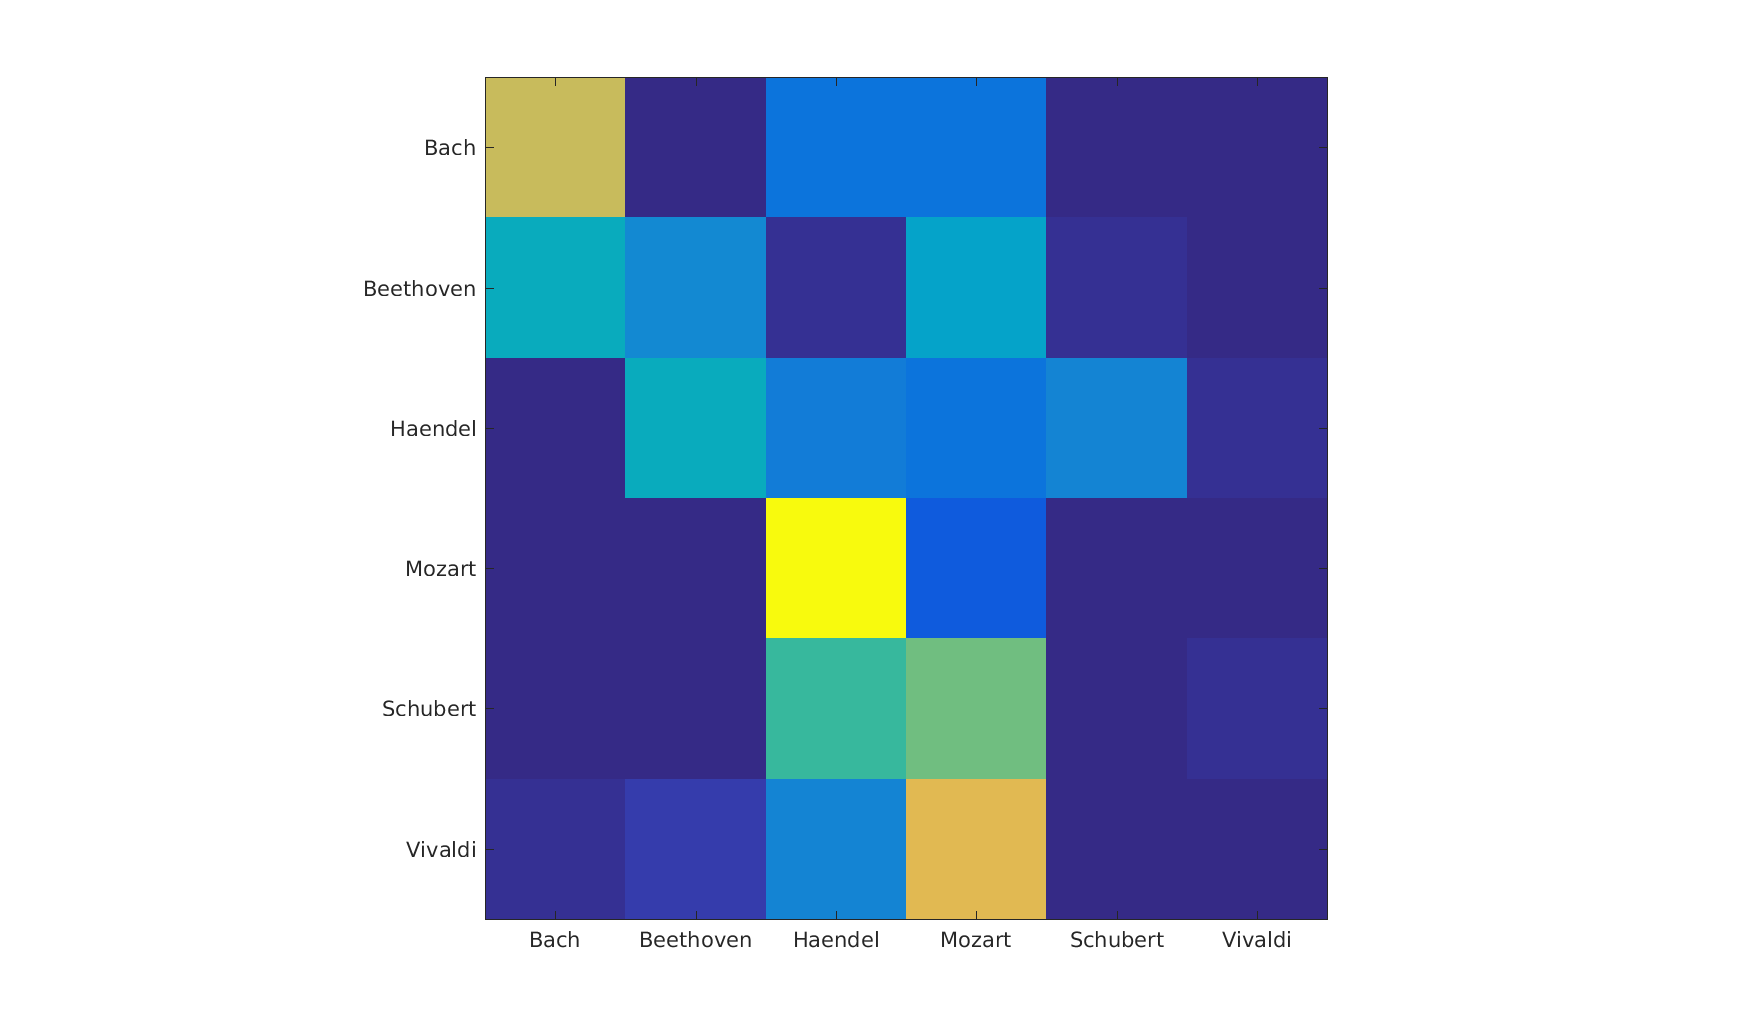
\includegraphics[scale=0.3]{misc/CM_st_7.png}
		\caption{Confusion matrices on both the datasets using k-NN with $k = \left[3,5,7\right]$}
	\end{figure}
	
	\section{Conclusions and future work}
	\lipsum[1-3]
	

\end{document}